\newpage
\section{Appendix Near-Infrared}
Infrared energy is electromagnetic energy from molecular vibration. It is invisible to the human eye. All objects emit some level of infrared radiation. When atoms absorb this energy, they produce the frequencies that release energy as IR.\\

The electromagnetic has a range of wavelengths, from shorter, near infrared waves to longer, far infrared waves. Near-Infrared waves are closer to visible light and do not emit detectable heat. As plants only use visible light for photosynthesis, infrared light and visible light can be compared to each other to estimate the amount of healthy vegetation. \cite{nasanir} This difference is usually expressed in a Normalized Difference Vegetation Index (NDVI) as follows:\\

\[NDVI = \frac{NIR-VIS}{NIR+VIS}\]

where
\begin{tabbing}
$NDVI$ = Normalized Difference Vegetation Index\\
$NIR$ = Near-Infrared\\
$VIS$ = Visible Light\\
\end{tabbing}

To record Near-Infrared (NIR), one could remove the infrared-blocking filter from a standard digital camera, and adding a color infrared film.

\begin{figure}[h]
\centering
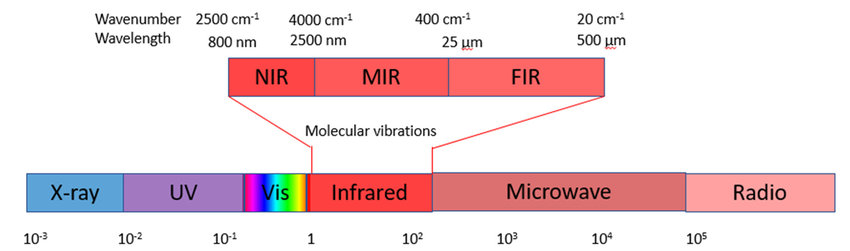
\includegraphics[scale=0.5]{appendix/b1_spectralrange.jpg}
\caption{Infrared spectral range \cite{infraredspectrum}}
\end{figure}

This can filters out the red or blue light, and measures infrared light in its place. Once a multi-spectral photograph is taken with a modified camera, one can post-process it, compositing the infrared and visible data to generate a new image which displays healthy, photo-synthetically active areas as bright regions. \cite{publiclabnir}

\subsubsection*{NDVI for drought conditions}
As seen by research done at Lake Victoria, there seems to be covariability between the water levels and NDVI. \cite{victorialake} The research concluded that NDVI can be used to identify human caused drought episodes.

